\section*{Appendix}
\addcontentsline{toc}{section}{Appendix}

\subsection{Web-Based Platform for Data Partitioning Evaluation}\label{subsec:web_platform}

\begin{figure*}
    \centering
    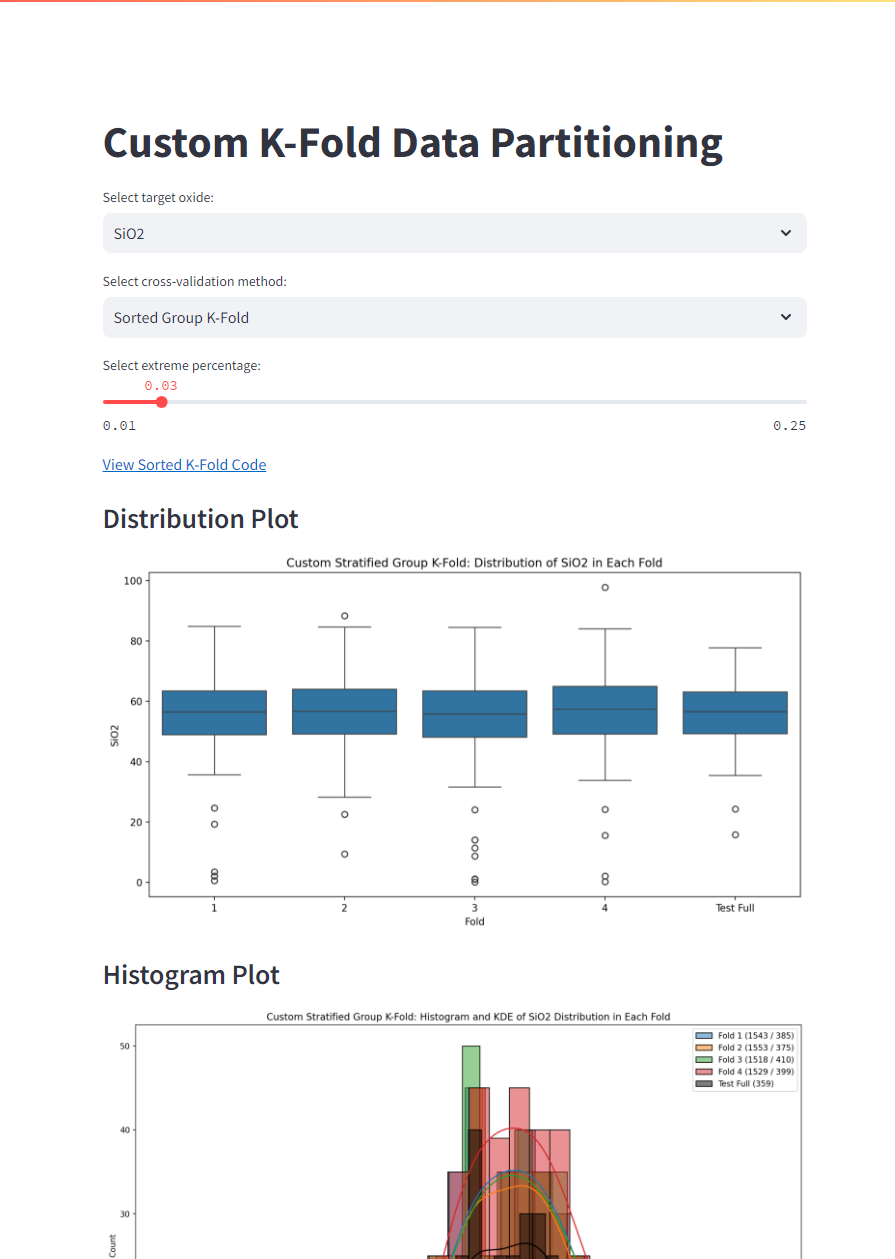
\includegraphics[width=\textwidth]{images/web_platform.png}
    \caption{Web-based platform used to determine the optimal value of $p$ for the data partitioning algorithm.}
    \label{fig:web_platform}
\end{figure*}

\subsection{Cross-Validation Plots for Major Oxides}\label{subsec:cv_plots}

% Loop through each major oxide and add a subsubsection with figures
\foreach \oxide in {SiO2, TiO2, Al2O3, FeOT, MgO, CaO, Na2O, K2O} {
    \subsubsection{\oxide}

    \begin{figure*}
        \centering
        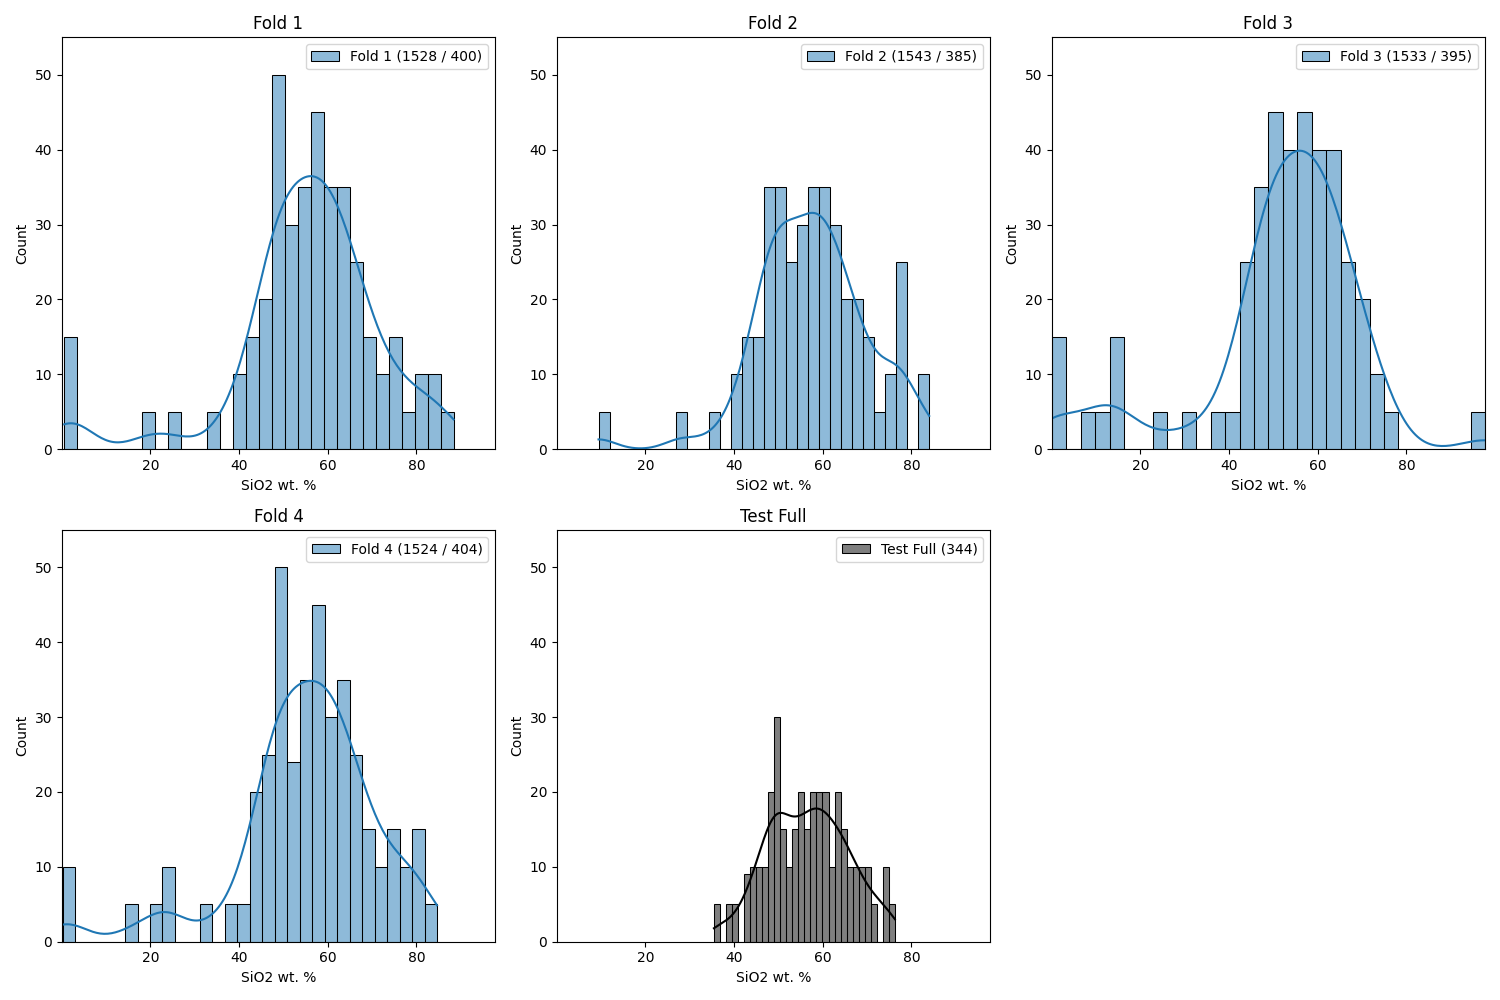
\includegraphics[width=\textwidth]{images/\oxide/histogram_grid_plot.png}
        \caption{Histogram and \gls{kde} of \ce{\oxide} distribution in each fold. The y-axis represents the count of samples per bin, and the x-axis represents \ce{\oxide} concentration. The notation in the legend indicates the amount of instances in the training/validation sets.}
        \label{fig:histogram_grid_plot_\oxide}
    \end{figure*}

    \begin{figure*}
        \centering
        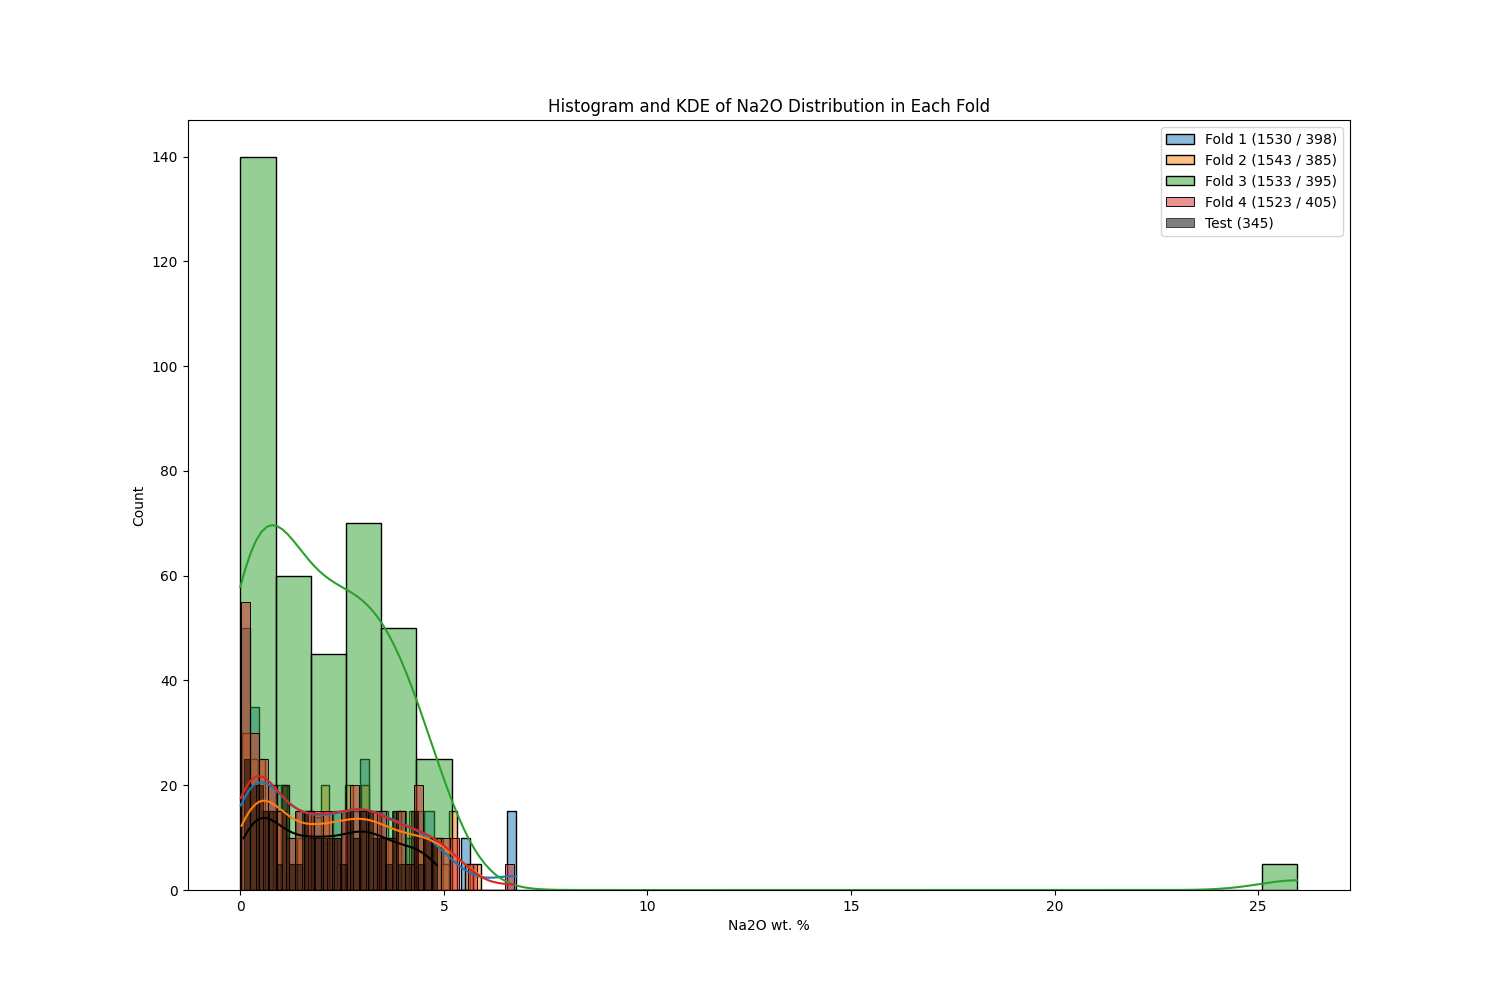
\includegraphics[width=\textwidth]{images/\oxide/histogram_kde_plot.png}
        \caption{Combined Histogram and \gls{kde} of \ce{\oxide} distribution in each fold. The y-axis represents the count of samples per bin, and the x-axis represents \ce{\oxide} concentration. The notation in the legend indicates the amount of instances in the training/validation sets.}
        \label{fig:histogram_kde_plot_\oxide}
    \end{figure*}

    \begin{figure*}
        \centering
        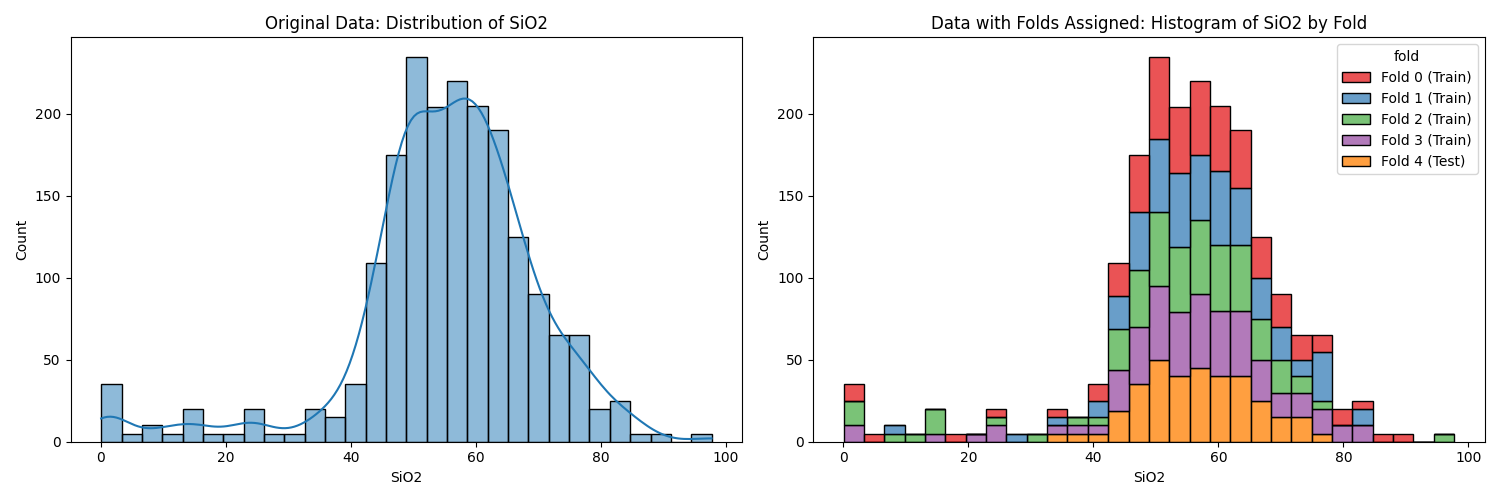
\includegraphics[width=\textwidth]{images/\oxide/original_and_post_fold.png}
        \caption{Distribution of \ce{\oxide} concentrations before and after fold assignment. The left plot shows the original distribution of \ce{\oxide}, while the right plot shows the distribution with folds assigned, color-coded to indicate the different folds.}
        \label{fig:original_and_post_fold_plot_\oxide}
    \end{figure*}

    \begin{figure*}
        \centering
        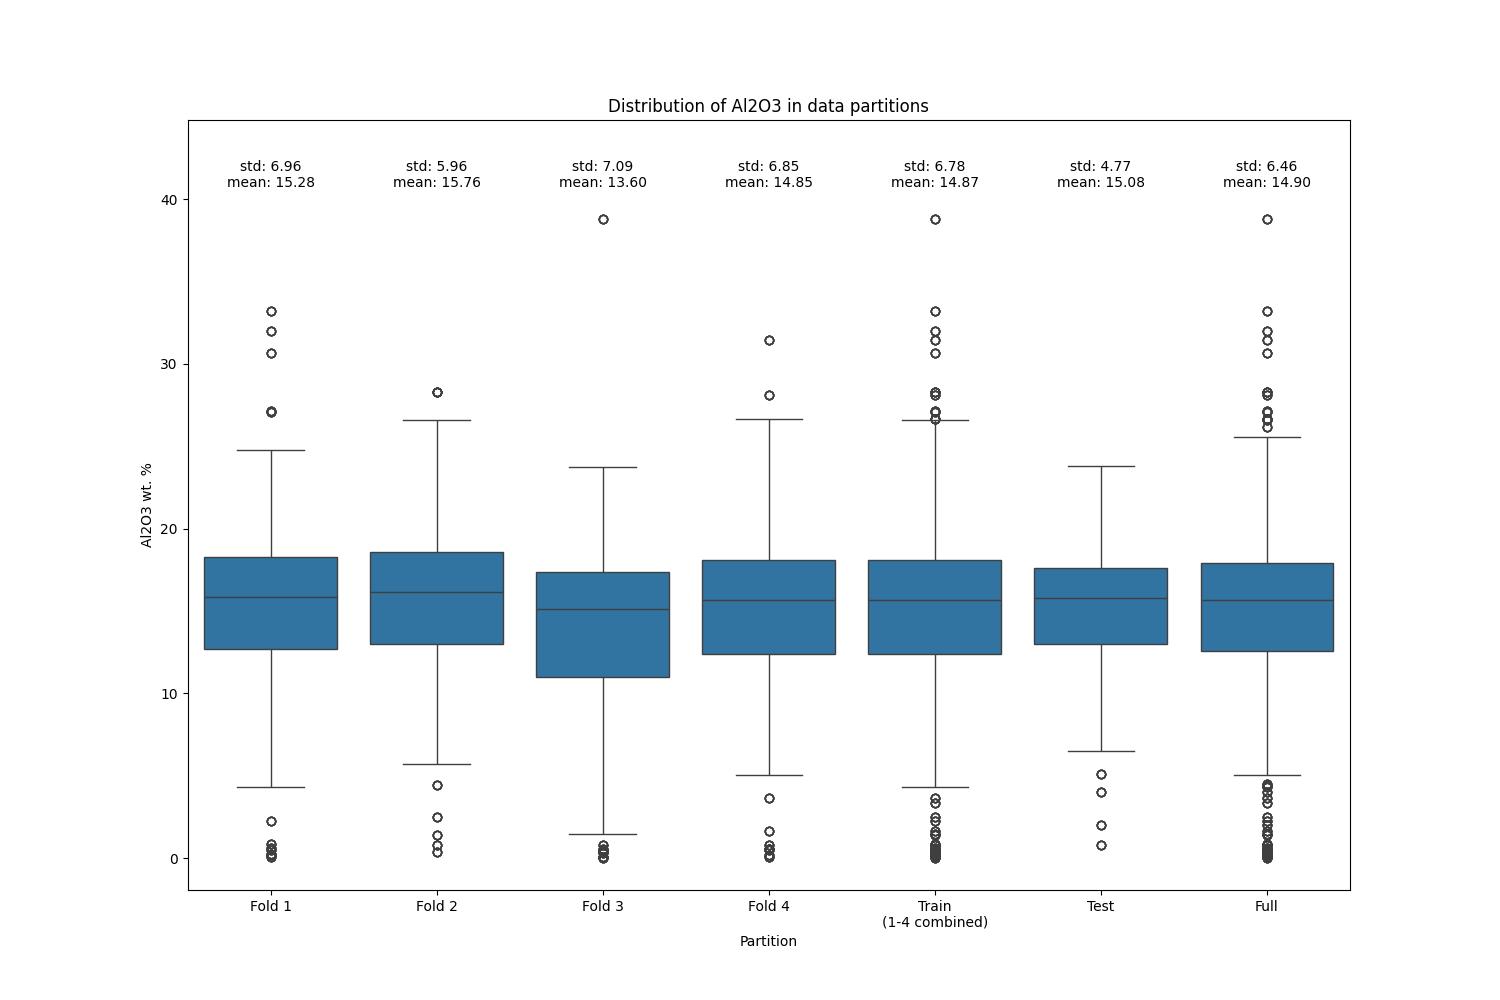
\includegraphics[width=\textwidth]{images/\oxide/distribution_plot.png}
        \caption{Distribution of \ce{\oxide} concentrations across cross-validation folds, training set, test set, and the entire dataset. The mean and standard deviation statistics for each partition are indicated figure.}
        \label{fig:distribution_plot_\oxide}
    \end{figure*}
}

\subsection{Initial Experiment: Model Hyperparameters}\label{subsec:initial_experiment_hyperparameters}
\begin{table*}
\centering
\begin{tabular}{@{}llp{0.5\textwidth}@{}}
\toprule
\textbf{Model} & \textbf{Hyperparameter} & \textbf{Value} \\
\midrule
\multirow{3}{*}{\gls{pls}}
& \texttt{n\_components} & 34 \\
& \texttt{scale} & True \\
& \texttt{max\_iter} & 500 \\
\midrule
\multirow{6}{*}{\gls{svr}}
& \texttt{kernel} & poly \\
& \texttt{C} & 100 \\
& \texttt{epsilon} & 0.1 \\
& \texttt{gamma} & scale \\
& \texttt{degree} & 2 \\
& \texttt{coef0} & 1.0 \\
\midrule
\multirow{3}{*}{Ridge Regression}
& \texttt{alphas} & \{$10^{-4}$, $10^{-3}$, $10^{-2}$, $10^{-1}$, 1, 10, $10^2$, $10^3$\} \\
& \texttt{max\_iter} & 1000 \\
& \texttt{tol} & $10^{-4}$ \\
\midrule
\multirow{3}{*}{\gls{lasso}}
& \texttt{alphas} & \{$10^{-4}$, $10^{-3}$, $10^{-2}$, $10^{-1}$, 1, 10, $10^2$, $10^3$\} \\
& \texttt{max\_iter} & 1000 \\
& \texttt{tol} & $10^{-4}$ \\
\midrule
\multirow{4}{*}{\gls{enet}}
& \texttt{alphas} & \{$10^{-4}$, $10^{-3}$, $10^{-2}$, $10^{-1}$, 1, 10, $10^2$, $10^3$\} \\
& \texttt{l1\_ratio} & \{0.1, 0.5, 0.7, 0.9, 1.0\} \\
& \texttt{max\_iter} & 1000 \\
& \texttt{tol} & $10^{-4}$ \\
\midrule
\multirow{6}{*}{\gls{rf}}
& \texttt{n\_estimators} & 100 \\
& \texttt{max\_depth} & 10 \\
& \texttt{min\_samples\_split} & 2 \\
& \texttt{min\_samples\_leaf} & 1 \\
& \texttt{max\_features} & sqrt \\
& \texttt{random\_state} & 42 \\
\midrule
\multirow{5}{*}{\gls{etr}}
& \texttt{n\_estimators} & 100 \\
& \texttt{max\_depth} & 10 \\
& \texttt{min\_samples\_split} & 2 \\
& \texttt{min\_samples\_leaf} & 1 \\
& \texttt{random\_state} & 42 \\
\midrule
\end{tabular}
\caption{Explictly set hyperparameters for the \gls{pls}, \gls{svr}, ridge, \gls{lasso}, \gls{enet}, \gls{rf}, and \gls{etr} models. When not explicitly set, the default hyperparameters provided by the libraries listed in Section~\ref{sec:experimental_setup} are used.}
\label{tab:combined_hyperparameters}
\end{table*}


\begin{table*}
\centering
\begin{tabular}{@{}llp{0.5\textwidth}@{}}
\toprule
\textbf{Model} & \textbf{Hyperparameter} & \textbf{Value} \\
\midrule
\multirow{14}{*}{\gls{gbr}}
& \texttt{n\_estimators} & 100 \\
& \texttt{max\_depth} & 3 \\
& \texttt{min\_samples\_split} & 2 \\
& \texttt{min\_samples\_leaf} & 1 \\
& \texttt{max\_features} & None \\
& \texttt{loss} & squared\_error \\
& \texttt{learning\_rate} & 0.1 \\
& \texttt{subsample} & 1.0 \\
& \texttt{criterion} & friedman\_mse \\
& \texttt{random\_state} & 42 \\
& \texttt{verbose} & 0 \\
& \texttt{validation\_fraction} & 0.1 \\
& \texttt{n\_iter\_no\_change} & None \\
& \texttt{tol} & $10^{-4}$ \\
& \texttt{ccp\_alpha} & 0.0 \\
\midrule
\gls{ngboost} & - & - \\
\midrule
\multirow{14}{*}{\gls{xgboost}}
& \texttt{max\_depth} & 4 \\
& \texttt{min\_child\_weight} & 5 \\
& \texttt{gamma} & 0.1 \\
& \texttt{subsample} & 0.7 \\
& \texttt{colsample\_bytree} & 0.5 \\
& \texttt{colsample\_bylevel} & 0.5 \\
& \texttt{colsample\_bynode} & 0.5 \\
& \texttt{lambda} & 1 \\
& \texttt{alpha} & 0.5 \\
& \texttt{learning\_rate} & 0.05 \\
& \texttt{n\_estimators} & 100 \\
& \texttt{objective} & reg:squarederror \\
& \texttt{eval\_metric} & rmse \\
\bottomrule
\end{tabular}
\caption{Explictly set hyperparameters for the \gls{gbr} and \gls{xgboost} models. When not explicitly set, the default hyperparameters provided by the libraries listed in Section~\ref{sec:experimental_setup} are used. The \gls{ngboost} model does not have any explicitly set hyperparameters.}
\label{tab:combined_hyperparameters}
\end{table*}

\begin{table*}
  \centering
  \begin{tabular}{lll}
    \toprule
    \textbf{Layer} & \textbf{Output Shape} & \textbf{Hyperparameter} \\ \midrule
    Input & (\textit{input\_dim},) & - \\
    Dense & (1024,) & activation = ReLU \\
    Dropout & (1024,) & rate = 0.3 \\
    Dense & (512,) & activation = ReLU \\
    Dropout & (512,) & rate = 0.3 \\
    Dense & (256,) & activation = ReLU \\
    Dense & (128,) & activation = ReLU \\
    Output & (\textit{output\_dim},) & - \\
    \midrule
    \multicolumn{3}{l}{\textbf{Optimizer:} Adam} \\
    \multicolumn{3}{l}{\textbf{Learning Rate:} 0.001} \\
    \bottomrule
  \end{tabular}
  \caption{Summary of the Neural Network Architecture}
  \label{tab:nn_architecture}
\end{table*}

\begin{table*}
  \centering
  \begin{tabular}{lll}
    \toprule
    \textbf{Layer} & \textbf{Output Shape} & \textbf{Hyperparameter} \\ \midrule
    Input & (\textit{input\_dim},) & - \\
    Reshape & (48, 128, 1) & - \\
    Conv2D & (48, 128, 32) & filters = 32, kernel\_size = (3, 3), activation = ReLU, padding = 'same' \\
    BatchNormalization & (48, 128, 32) & - \\
    MaxPooling2D & (24, 64, 32) & pool\_size = (2, 2) \\ \midrule

    Conv2D & (24, 64, 32) & filters = 32, kernel\_size = (3, 3), activation = ReLU, padding = 'same' \\
    BatchNormalization & (24, 64, 32) & - \\
    MaxPooling2D & (12, 32, 32) & pool\_size = (2, 2) \\ \midrule

    Conv2D & (12, 32, 64) & filters = 64, kernel\_size = (3, 3), activation = ReLU, padding = 'same' \\
    BatchNormalization & (12, 32, 64) & - \\
    MaxPooling2D & (6, 16, 64) & pool\_size = (2, 2) \\ \midrule

    Conv2D & (6, 16, 128) & filters = 128, kernel\_size = (3, 3), activation = ReLU, padding = 'same' \\
    BatchNormalization & (6, 16, 128) & - \\
    MaxPooling2D & (3, 8, 128) & pool\_size = (2, 2) \\ \midrule

    Flatten & (3072,) & - \\
    Dense & (256,) & activation = ReLU \\
    Dropout & (256,) & rate = 0.5 \\
    Dense & (\textit{output\_dim},) & - \\
    Dense & (\textit{output\_dim},) & kernel\_regularizer = $L_2(0.01)$ \\ \midrule
    \multicolumn{3}{l}{\textbf{Optimizer:} Adam} \\
    \multicolumn{3}{l}{\textbf{Learning Rate:} 0.001} \\
    \bottomrule
  \end{tabular}
  \caption{Summary of the Convolutional Neural Network Architecture}
  \label{tab:cnn_architecture}
\end{table*}
